\documentclass[10pt,twocolumn,twoside,slovak,a4paper]{article}

\usepackage{amsmath}
\usepackage{graphicx}
\usepackage{subcaption}
\usepackage{wrapfig}

\begin{document}

\begin{figure}
 \centering
\begin{subfigure} {.5\textwidth}
  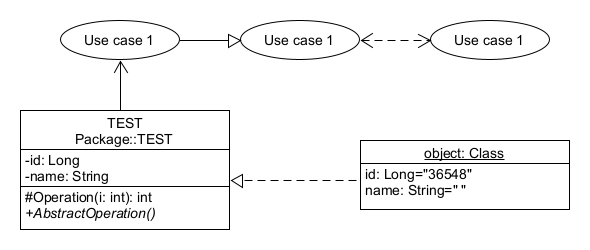
\includegraphics[width=\linewidth]{diag1.png}
  \caption{Diagram 1}
\end{subfigure}%
\begin{subfigure} {.5\textwidth}
  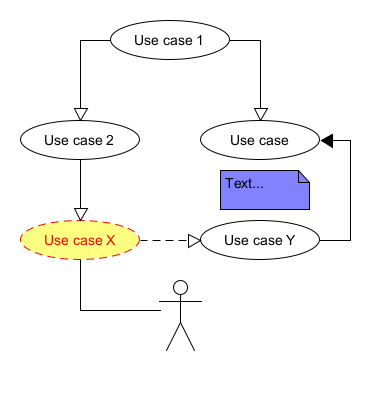
\includegraphics[width=\linewidth]{diag2.png}
  \caption{Diagram 2}
\end{subfigure}
\end{figure}

\begin{figure*}
  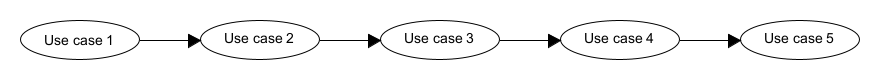
\includegraphics[width=\textwidth]{diag3.png}
  \caption[width=\textwidth]{Diagram 3}
\end{figure*}

\clearpage
\clearpage


Lorem ipsum dolor sit amet, consectetur adipiscing elit. Quisque scelerisque erat quis pharetra pharetra. Donec id nulla at elit aliquam placerat non in justo. Curabitur lobortis, odio et fringilla accumsan, nibh sem rhoncus velit, eu efficitur quam dui sit amet tortor. Cras ultricies magna non nisi dictum blandit. Proin pellentesque arcu orci, sit amet tincidunt neque sagittis non. Sed pretium dui non lectus dapibus convallis.
\begin{wrapfigure}{l}{0.35\textwidth}
    
\includegraphics[width=\linewidth]{STU-FIIT-zfv.png}
\end{wrapfigure}
Mauris eu ex ipsum. Quisque feugiat orci condimentum enim congue volutpat. Vivamus placerat tincidunt faucibus. Pellentesque ut sollicitudin lorem, quis ornare odio. Vivamus in magna accumsan, interdum arcu sed, venenatis nibh. In hac habitasse platea dictumst. Nullam vel accumsan nunc. Sed convallis felis ac turpis suscipit, eget placerat odio blandit. Integer non luctus diam. Fusce eu ullamcorper neque.

\clearpage

$\begin{matrix}
1 & 2 & 3 & 4 & 5\\
1 & 2 & 3 & 4 & 5\\
1 & 2 & 3 & 4 & 5\\
1 & 2 & 3 & 4 & 5\\
1 & 2 & 3 & 4 & 5
\end{matrix}$


\end{document}